\documentclass[../main.tex]{subfiles}
\begin{document}
\part*{Infrastructure}
The infrastructure described is a common architecture for building web applications that require image recognition capabilities. The infrastructure is divided into two tiers: the Web Tier and the Application Tier.

The Web Tier is responsible for interacting with users and displaying the user interface. It uses HTML/JS/CSS to render the interface and collects user inputs. In this architecture, a Python Flask is used for user interaction.

The Application Tier is the core of the application and performs the image recognition tasks. It handles business logic, database manipulation functions (CRUD), and communicates with other resources. In this architecture, an AWS Deep Learning model is used for image classification.

\begin{figure}[h!]
\centering
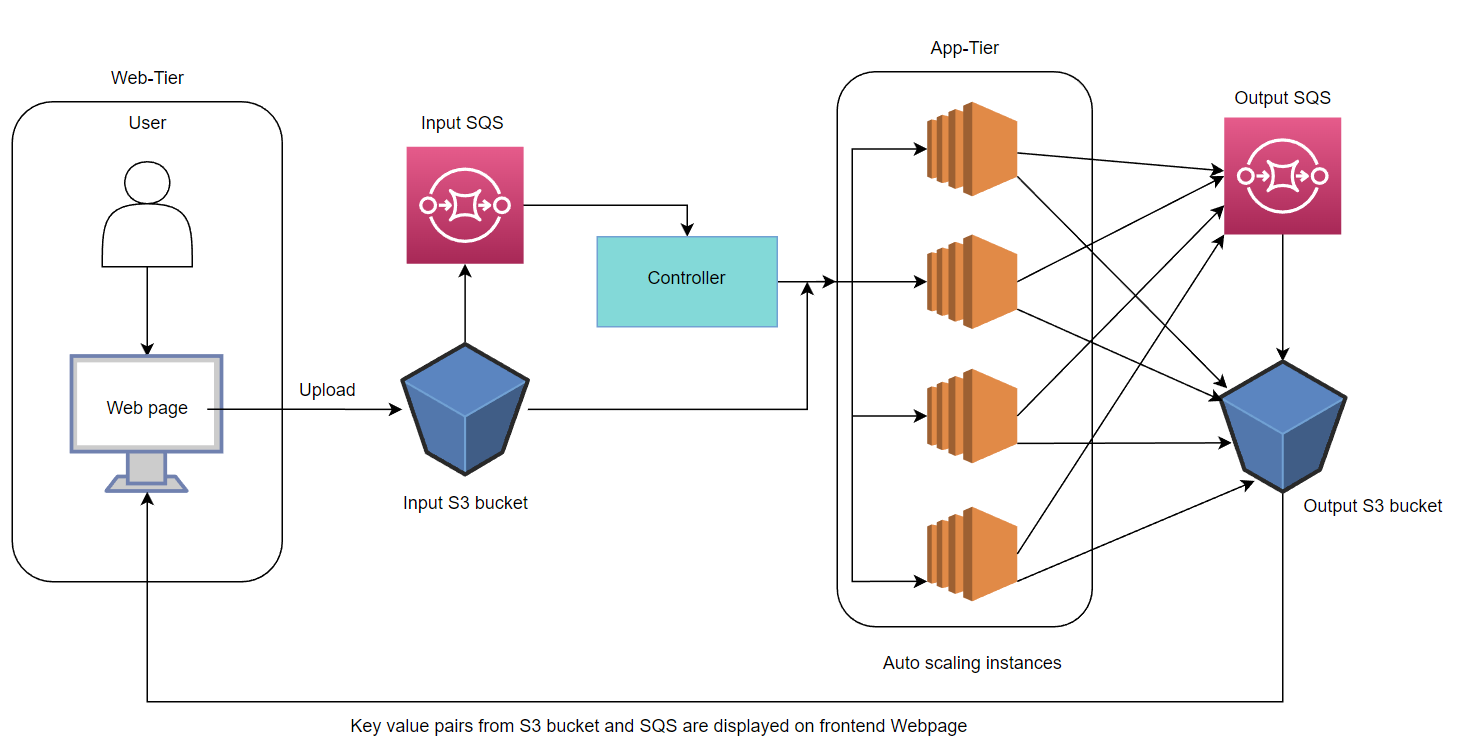
\includegraphics[scale=0.8]{images/arc.png}
\caption{System Architecture. (working on it)}
\label{fig:im_uses}
\end{figure}

The resources used in this infrastructure include input and output S3 buckets for loading images and displaying classified images on the user interface. The App Tier uses SQS for input images as messages and stores them for processing. The classified image results are then passed onto the output SQS and then onto the output S3 bucket, which is then used by the Web Tier to display the classified images on the user interface.

The number of EC2 instances to be used depends on the amount data uploaded. In case if we upload images less than 15 then the number of instances running will be equal to the number of images uploaded.

Overall, this infrastructure provides a scalable and cost-effective way to build web applications with image recognition capabilities. By separating the Web and Application Tiers and using AWS services, the infrastructure can automatically scale resources up or down based on demand, improving performance and reducing costs.

\end{document}

\clearpage